\documentclass[dvipdfmx]{jsarticle}
\setcounter{section}{1}
\setcounter{subsection}{9}
\usepackage{amsmath,amsfonts,amssymb,array,comment,mathtools,url,docmute}
\usepackage{longtable,booktabs,dcolumn,tabularx,mathtools,multirow,colortbl,xcolor}
\usepackage[dvipdfmx]{graphics}
\usepackage{bmpsize}
\usepackage{amsthm}
\usepackage{enumitem}
\setlistdepth{20}
\renewlist{itemize}{itemize}{20}
\setlist[itemize]{label=•}
\renewlist{enumerate}{enumerate}{20}
\setlist[enumerate]{label=\arabic*.}
\setcounter{MaxMatrixCols}{20}
\setcounter{tocdepth}{3}
\newcommand{\rotin}{\text{\rotatebox[origin=c]{90}{$\in $}}}
\newcommand{\amap}[6]{\text{\raisebox{-0.7cm}{\begin{tikzpicture} 
  \node (a) at (0, 1) {$\textstyle{#2}$};
  \node (b) at (#6, 1) {$\textstyle{#3}$};
  \node (c) at (0, 0) {$\textstyle{#4}$};
  \node (d) at (#6, 0) {$\textstyle{#5}$};
  \node (x) at (0, 0.5) {$\rotin $};
  \node (x) at (#6, 0.5) {$\rotin $};
  \draw[->] (a) to node[xshift=0pt, yshift=7pt] {$\textstyle{\scriptstyle{#1}}$} (b);
  \draw[|->] (c) to node[xshift=0pt, yshift=7pt] {$\textstyle{\scriptstyle{#1}}$} (d);
\end{tikzpicture}}}}
\newcommand{\twomaps}[9]{\text{\raisebox{-0.7cm}{\begin{tikzpicture} 
  \node (a) at (0, 1) {$\textstyle{#3}$};
  \node (b) at (#9, 1) {$\textstyle{#4}$};
  \node (c) at (#9+#9, 1) {$\textstyle{#5}$};
  \node (d) at (0, 0) {$\textstyle{#6}$};
  \node (e) at (#9, 0) {$\textstyle{#7}$};
  \node (f) at (#9+#9, 0) {$\textstyle{#8}$};
  \node (x) at (0, 0.5) {$\rotin $};
  \node (x) at (#9, 0.5) {$\rotin $};
  \node (x) at (#9+#9, 0.5) {$\rotin $};
  \draw[->] (a) to node[xshift=0pt, yshift=7pt] {$\textstyle{\scriptstyle{#1}}$} (b);
  \draw[|->] (d) to node[xshift=0pt, yshift=7pt] {$\textstyle{\scriptstyle{#2}}$} (e);
  \draw[->] (b) to node[xshift=0pt, yshift=7pt] {$\textstyle{\scriptstyle{#1}}$} (c);
  \draw[|->] (e) to node[xshift=0pt, yshift=7pt] {$\textstyle{\scriptstyle{#2}}$} (f);
\end{tikzpicture}}}}
\renewcommand{\thesection}{第\arabic{section}部}
\renewcommand{\thesubsection}{\arabic{section}.\arabic{subsection}}
\renewcommand{\thesubsubsection}{\arabic{section}.\arabic{subsection}.\arabic{subsubsection}}
\everymath{\displaystyle}
\allowdisplaybreaks[4]
\usepackage{vtable}
\theoremstyle{definition}
\newtheorem{thm}{定理}[subsection]
\newtheorem*{thm*}{定理}
\newtheorem{dfn}{定義}[subsection]
\newtheorem*{dfn*}{定義}
\newtheorem{axs}[dfn]{公理}
\newtheorem*{axs*}{公理}
\renewcommand{\headfont}{\bfseries}
\makeatletter
  \renewcommand{\section}{%
    \@startsection{section}{1}{\z@}%
    {\Cvs}{\Cvs}%
    {\normalfont\huge\headfont\raggedright}}
\makeatother
\makeatletter
  \renewcommand{\subsection}{%
    \@startsection{subsection}{2}{\z@}%
    {0.5\Cvs}{0.5\Cvs}%
    {\normalfont\LARGE\headfont\raggedright}}
\makeatother
\makeatletter
  \renewcommand{\subsubsection}{%
    \@startsection{subsubsection}{3}{\z@}%
    {0.4\Cvs}{0.4\Cvs}%
    {\normalfont\Large\headfont\raggedright}}
\makeatother
\makeatletter
\renewenvironment{proof}[1][\proofname]{\par
  \pushQED{\qed}%
  \normalfont \topsep6\p@\@plus6\p@\relax
  \trivlist
  \item\relax
  {
  #1\@addpunct{.}}\hspace\labelsep\ignorespaces
}{%
  \popQED\endtrivlist\@endpefalse
}
\makeatother
\renewcommand{\proofname}{\textbf{証明}}
\usepackage{tikz,graphics}
\usepackage[dvipdfmx]{hyperref}
\usepackage{pxjahyper}
\hypersetup{
 setpagesize=false,
 bookmarks=true,
 bookmarksdepth=tocdepth,
 bookmarksnumbered=true,
 colorlinks=false,
 pdftitle={},
 pdfsubject={},
 pdfauthor={},
 pdfkeywords={}}
\begin{document}
%\hypertarget{ux7f6eux63db}{%
\subsection{置換}%\label{ux7f6eux63db}}
%\hypertarget{ux7f6eux63db-1}{%
\subsubsection{置換}%\label{ux7f6eux63db-1}}
\begin{dfn}
添数集合$\varLambda_{n}$について考えよう。次のような写像$p$をその添数集合$\varLambda_{n}$の置換といい$\begin{pmatrix}
(i)_{i \in \varLambda_{n}} \\
\left( p(i) \right)_{i \in \varLambda_{n}} \\
\end{pmatrix}$とも書く。
\begin{align*}
p:\varLambda_{n}\overset{\sim}{\rightarrow}\varLambda_{n};i \mapsto p(i)
\end{align*}
2つの置換たち$p$、$p'$が与えられたとき、その置換$p$を$\begin{pmatrix}
\left( p'(i) \right)_{i \in \varLambda_{n}} \\
\left( p \circ p'(i) \right)_{i \in \varLambda_{n}} \\
\end{pmatrix}$と書いてもよい。また、添数集合$\varLambda_{n}$の置換全体の集合$\mathfrak{S}_{n}$を置換群という。
\end{dfn}
\begin{thm}\label{2.1.10.1}
置換群$\mathfrak{S}_{n}$について、${\#}\mathfrak{S}_{n} = n!$が成り立つ。
\end{thm}
\begin{proof}
置換群$\mathfrak{S}_{n}$について、$n = 1$のときは明らかに${\#}\mathfrak{S}_{1} = 1!$が成り立つ。\par
ここで、$n = k$のとき、${\#}\mathfrak{S}_{k} = k!$が成り立つと仮定しよう。$n = k + 1$のとき、残りの元々の集合$\varLambda_{k + 1} \setminus \left\{ k + 1 \right\}$は添数集合$\varLambda_{k}$に等しく写像$p|\varLambda_{k}:\varLambda_{k}\overset{\sim}{\rightarrow}\varLambda_{k + 1} \setminus \left\{ p(k + 1) \right\}$を考えよう。$\forall i' \in \varLambda_{k}$に対し、次式のように集合たち$\mathfrak{F}$、$\mathfrak{R}_{i'}$と
\begin{align*}
\mathfrak{F} &= \left\{ p|\varLambda_{k}\in \mathfrak{F}\left( \varLambda_{k},\varLambda_{k + 1} \setminus \left\{ p(k + 1) \right\} \right) \middle| p:\varLambda_{k + 1}\overset{\sim}{\rightarrow}\varLambda_{k + 1} \right\}\\
&\mathfrak{R}_{i'} = \left\{ p \in \mathfrak{F}\left( \varLambda_{k + 1},\varLambda_{k + 1} \right) \middle| p(k + 1) = i' \right\}
\end{align*}
次式のような写像$\mathfrak{p}(p)$が定められよう。
\begin{align*}
\mathfrak{p:}\mathfrak{R}_{i'}\mathfrak{\rightarrow F;}p \mapsto \mathfrak{p}(p) = p|\varLambda_{k}:\varLambda_{k} \rightarrow \varLambda_{k + 1} \setminus \left\{ p(k + 1) \right\};i \mapsto p(i)
\end{align*}
定義より$\mathfrak{p}(p) = \mathfrak{p}(q)$が成り立つなら、明らかに$p = q$が成り立つかつ、$p' \in \mathfrak{S}_{k} \setminus V\left( \mathfrak{p} \right)$なる写像$p'$が存在したと仮定すると、次のように写像$p''$を考えれば、
\begin{align*}
p'':\varLambda_{k + 1} \rightarrow \varLambda_{k + 1};i \mapsto \left\{ \begin{matrix}
i' & \mathrm{if} & i = k + 1 \\
p'(i) & \mathrm{if} & i \neq k + 1 \\
\end{matrix} \right.\ 
\end{align*}
写像$\mathfrak{p}\left( p'' \right)$は次のようになる。
\begin{align*}
\mathfrak{p}\left( p'' \right) = p''|\varLambda_{k}:\varLambda_{k} \rightarrow \varLambda_{k + 1} \setminus \left\{ p''(k + 1) \right\};i \mapsto p''(i)
\end{align*}
ここで、$\forall i \in D\left( \mathfrak{p}\left( p'' \right) \right) = \varLambda_{k}$に対し、次のようになるが、
\begin{align*}
\mathfrak{p}\left( p'' \right)(i) = p''(i) = p'(i)
\end{align*}
これは$p' \in \mathfrak{S}_{k} \setminus V\left( \mathfrak{p} \right)$が成り立つことに矛盾する。したがって、その写像$\mathfrak{p}$は全単射である。ゆえに、その自然数$i'$によらず${\#}\mathfrak{R}_{i'} = {\#}\mathfrak{F}$が成り立つ。また、その写像$p$は単射であるから、次式のような写像$\mathfrak{p}'$が考えられることができる。
\begin{align*}
\mathfrak{p}'\mathfrak{:F \rightarrow}\mathfrak{S}_{k};p \mapsto \mathfrak{p}(p):\varLambda_{k}\overset{\sim}{\rightarrow}\varLambda_{k};i \mapsto \left\{ \begin{matrix}
p(k + 1) & \mathrm{if} & p(i) = k + 1 \\
p(i) & \mathrm{if} & p(i) \neq k + 1 \\
\end{matrix} \right.\ 
\end{align*}
定義より$\mathfrak{p}'(p) = \mathfrak{p}'(q)$が成り立つなら、明らかに$p = q$が成り立つかつ、$p' \in \mathfrak{S}_{k} \setminus V\left( \mathfrak{p}' \right)$なる写像$p'$が存在したと仮定すると、$i' \in \varLambda_{k}$なる自然数$i'$を選んで次のように写像$p''$を考えれば、
\begin{align*}
p'':\varLambda_{k + 1}\overset{\sim}{\rightarrow}\varLambda_{k + 1};i \mapsto \left\{ \begin{matrix}
k + 1 & \mathrm{if} & i = i' \\
p'\left( i' \right) & \mathrm{if} & i = k + 1 \\
p'(i) & \mathrm{if} & i \neq i' \land i \neq k + 1 \\
\end{matrix} \right.\ 
\end{align*}
写像$\mathfrak{p}'\left( p'' \right)$は次のようになり
\begin{align*}
\mathfrak{p}'\left( p'' \right):\varLambda_{k}\overset{\sim}{\rightarrow}\varLambda_{k};i \mapsto \left\{ \begin{matrix}
p''(k + 1) & \mathrm{if} & p''(i) = k + 1 \\
p''(i) & \mathrm{if} & p''(i) \neq k + 1 \\
\end{matrix} \right.\ 
\end{align*}
ここで、$\forall i \in D\left( \mathfrak{p}'\left( p'' \right) \right) = \varLambda_{k}$に対し、次のようになるが、
\begin{align*}
\mathfrak{p}'\left( p'' \right)(i) &= \left\{ \begin{matrix}
p''(k + 1) & \mathrm{if} & p''(i) = k + 1 \\
p''(i) & \mathrm{if} & p''(i) \neq k + 1 \\
\end{matrix} \right.\ \\
&= \left\{ \begin{matrix}
p'\left( i' \right) & \mathrm{if} & i = i' \\
p'(i) & \mathrm{if} & i \neq i' \\
\end{matrix} \right. = p'(i)
\end{align*}
これは$p' \in \mathfrak{S}_{k} \setminus V\left( \mathfrak{p}' \right)$が成り立つことに矛盾する。したがって、その写像$\mathfrak{p}'$は全単射である。ゆえに、${\#}\mathfrak{F} = {\#}\mathfrak{S}_{k} = k!$が成り立つ。以上の関係が図式で表されると、次のようになる。
\begin{center}
  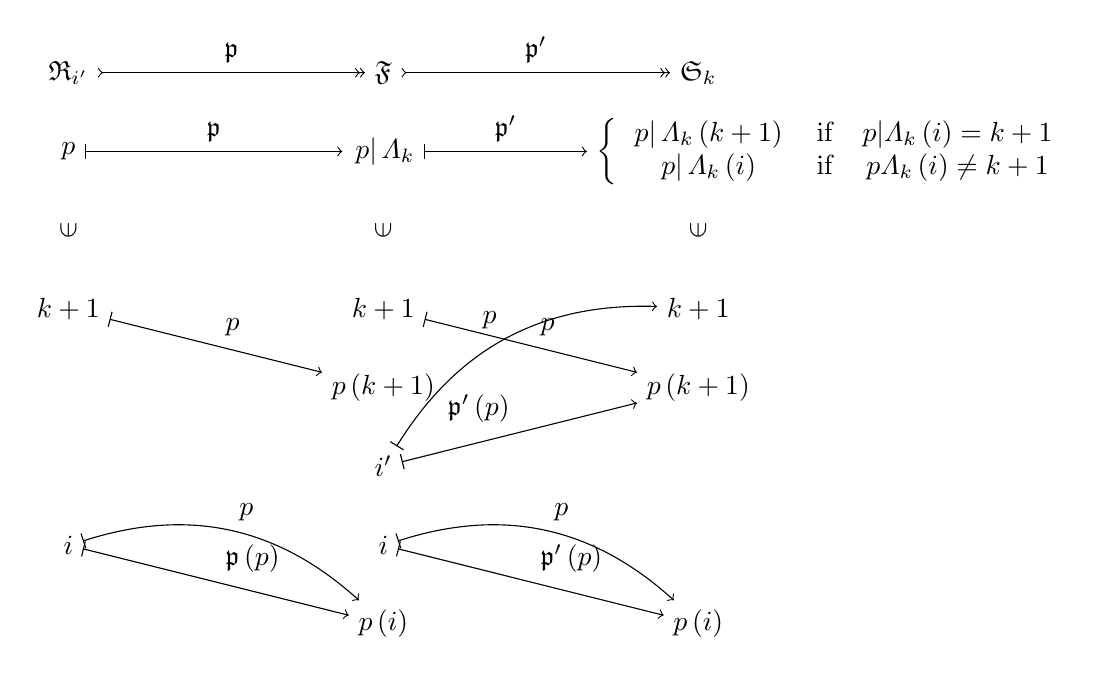
\begin{tikzpicture}[auto]

    \node (a) at (0, 7) {${\mathfrak R}_{i'} $};
    \node (b) at (4, 7) {${\mathfrak F} $};
    \node (c) at (8, 7) {${\mathfrak S}_k $};
    \node (d) at (0, 6) {$p$};
    \node (e) at (4, 6) {$\left. p\right|{\varLambda_k } $};
    \node (f) at (8, 6) {$\left\{ \begin{array}{c} \left. p\right|{\varLambda_k } \left( k+1\right) \\ \left. p\right|{\varLambda_k } \left( i\right) \end{array} \right. $};
    \node (f') at (11, 6) {$\begin{array}{cc} {\rm if} & p| \varLambda_k \left( i\right) =k+1\\ {\rm if} & p \varLambda_k \left( i\right) \neq k+1 \end{array} $};
    \draw [>->>] (a) to node {${\mathfrak p} $} (b);
    \draw [>->>] (b) to node {${\mathfrak p}' $} (c);
    \draw [|->] (d) to node {${\mathfrak p} $} (e);
    \draw [|->] (e) to node {${\mathfrak p}' $} (f);

    \node (x) at (0, 5) {\rotatebox{90}{$\in $}};
    \node (x) at (4, 5) {\rotatebox{90}{$\in $}};
    \node (x) at (8, 5) {\rotatebox{90}{$\in $}};

    \node (a) at (0, 1) {$i$};
    \node (b) at (4, 0) {$p\left( i\right) $};
    \node (c) at (8, 0) {$p\left( i\right) $};
    \node (d) at (4, 1) {$i$};
    \node (e) at (4, 2) {$i'$};
    \node (f) at (4, 3) {$p\left( k+1\right) $};
    \node (g) at (8, 3) {$p\left( k+1\right) $};
    \node (h) at (0, 4) {$k+1$};
    \node (i) at (4, 4) {$k+1$};
    \node (j) at (8, 4) {$k+1$};
    \draw [|->] (a) to[bend left=30] node {$p$} (b);
    \draw [|->] (a) to node {${\mathfrak p}\left( p\right) $} (b);
    \draw [|->] (d) to[bend left=30] node {$p$} (c);
    \draw [|->] (d) to node {${\mathfrak p}'\left( p\right) $} (c);
    \draw [|->] (e) to[bend left=30] node {$p$} (j);
    \draw [|->] (e) to node {${\mathfrak p}'\left( p\right) $} (g);
    \draw [|->] (h) to node {$p$} (f);
    \draw [|->] (i) to node {$p$} (g);

  \end{tikzpicture} 
\end{center}
また、その置換群$\mathfrak{S}_{k + 1}$は$\mathfrak{S}_{k + 1} = \bigsqcup_{i \in \varLambda_{k + 1}} \mathfrak{R}_{i}$のように書き換えられることができるので、したがって、次のようになる。
\begin{align*}
{\#}\mathfrak{S}_{k + 1} &= {\#}{\bigsqcup_{i \in \varLambda_{k + 1}} \mathfrak{R}_{i}}\\
&= {\#}\varLambda_{k + 1}{\#}\mathfrak{F}\\
&= {\#}\varLambda_{k + 1}{\#}\mathfrak{S}_{k}\\
&= (k + 1)k!\\
&= (k + 1)!
\end{align*}
よって、数学的帰納法によって${\#}\mathfrak{S}_{n} = n!$が成り立つことが示された。
\end{proof}
\begin{thm}\label{2.1.10.2}
定義より次のような恒等写像$I_{\varLambda_{n}}$もまたその添数集合$\varLambda_{n}$の置換となるかつ、
\begin{align*}
I_{\varLambda_{n}}:\varLambda_{n} \rightarrow \varLambda_{n};i \mapsto i
\end{align*}
$\forall p \in \mathfrak{S}_{n}$に対し、その置換$p$は全単射であるから、これの逆写像$p^{- 1}$が存在することに注意すれば、組$\left( \mathfrak{S}_{n}, \circ \right)$は群をなす。
\end{thm}
\begin{dfn}
置換の合成写像のことを置換の積、このときの恒等写像$I_{\varLambda_{n}}$のことを恒等置換、置換の逆写像のことを逆置換という。
\end{dfn}
\begin{proof}
置換群$\mathfrak{S}_{n}$について、置換同士の合成写像も置換であり、その集合$\mathfrak{S}_{n}$の元々は写像であるので、$\forall p,q,r \in \mathfrak{S}_{n}$に対し、次式が成り立つ。
\begin{align*}
(p \circ q) \circ r = p \circ (q \circ r)
\end{align*}
また、$\forall p \in \mathfrak{S}_{n}$に対し、次のような恒等写像$I_{\varLambda_{n}}$もまたその添数集合$\varLambda_{n}$の置換となるので、
\begin{align*}
I_{\varLambda_{n}}:\varLambda_{n} \rightarrow \varLambda_{n};i \mapsto i
\end{align*}
次式が成り立つような写像$I_{\varLambda_{n}}$がその置換群$\mathfrak{S}_{n}$に存在する。
\begin{align*}
I_{\varLambda_{n}} \circ p = p \circ I_{\varLambda_{n}} = p
\end{align*}
$\forall p \in \mathfrak{S}_{n}$に対し、その置換$p$は全単射でありこれの逆写像$p^{- 1}$が存在するので、次式が成り立つようなその写像$p$の逆元$p^{- 1}$が存在する。
\begin{align*}
p \circ p^{- 1} = p^{- 1} \circ p = I_{\varLambda_{n}}
\end{align*}
\end{proof}
\begin{dfn}
$n \geq 2$のとき、置換群$\mathfrak{S}_{n}$について、$i',j' \in \varLambda_{n}$なる互いに異なる元々$i'$、$j'$を選びその置換群$\mathfrak{S}_{n}$に属し次式が成り立つような置換$\tau$を考えよう。
\begin{align*}
\tau:\varLambda_{n} \rightarrow \varLambda_{n};i \mapsto \left\{ \begin{matrix}
j' & \mathrm{if} & i = j' \\
i' & \mathrm{if} & i = i' \\
i & \mathrm{if} & i \neq i' \land i \neq j' \\
\end{matrix} \right.\ 
\end{align*}
このような置換$\tau$をその添数集合$\varLambda_{n}$の互換といい$\begin{pmatrix}
i' & j' \\
\end{pmatrix}$などと書く。また、その添数集合$\varLambda_{n}$の互換$\tau$全体の集合を$\mathfrak{T}_{n}$とおく。
\end{dfn}\par
このとき、明らかに$\tau^{- 1} = \tau$が成り立つ。
\begin{thm}\label{2.1.10.3}
$n \geq 2$が成り立つなら、置換群$\mathfrak{S}_{n}$について、$\forall p \in \mathfrak{S}_{n}$に対し$\forall i \in \varLambda_{s}$に対し$\tau_{i} \in \mathfrak{T}_{k}$なる互換たち$\tau_{i}$を用いて次式のように表されることができる。\begin{align*}
p = \tau_{s} \circ \cdots \circ \tau_{2} \circ \tau_{1}
\end{align*}
\end{thm}\par
ただし、この表し方は一意的でないことに注意されたい。
\begin{proof}
置換群$\mathfrak{S}_{n}$について、$\forall p \in \mathfrak{S}_{n}$に対し$n = 2$のときその置換$p$自身が互換となる。\par
$n = k$のとき、$i \in \varLambda_{s}$なる互換たち$\tau_{i}$を用いて次式のように表されることができると仮定しよう。
\begin{align*}
p = \tau_{s} \circ \cdots \circ \tau_{2} \circ \tau_{1}
\end{align*}
$n = k + 1$のとき、$p(k + 1) = k + 1$が成り立つなら、その置換$p$を用いれば、次式のような写像$p'$が得られることができる。
\begin{align*}
p':\varLambda_{k} \rightarrow \varLambda_{k};i \mapsto p(i)
\end{align*}
その写像$p'$は明らかに$p' \in \mathfrak{S}_{k}$が成り立つので、仮定より$\forall i \in \varLambda_{s}$に対し$\tau_{i} \in \mathfrak{T}_{k + 1}$なる互換たち$\tau_{i}$を用いて次式のように表されることができる。
\begin{align*}
p' = \tau_{s} \circ \cdots \circ \tau_{2} \circ \tau_{1}
\end{align*}
このとき、次のような写像$\mathfrak{t}$を考えよう。
\begin{align*}
\mathfrak{t:}\mathfrak{T}_{k} \rightarrow \mathfrak{T}_{k + 1};\tau \mapsto \mathfrak{t}(\tau):\varLambda_{k + 1} \rightarrow \varLambda_{k + 1};i \mapsto \left\{ \begin{matrix}
k + 1 & \mathrm{if} & i = k + 1 \\
\tau(i) & \mathrm{if} & i \neq k + 1 \\
\end{matrix} \right.\ 
\end{align*}
このとき、$\forall i \in \varLambda_{k}$に対し$\tau(i) = \mathfrak{t}(\tau)(i)$が成り立つかつ、$\forall\tau \in \mathfrak{T}_{k}$に対し$\mathfrak{t}(\tau)(k + 1) = k + 1$が成り立つので、次のようになる。
\begin{align*}
p(i) &= \left\{ \begin{matrix}
k + 1 & \mathrm{if} & i = k + 1 \\
p'(i) & \mathrm{if} & i \neq k + 1 \\
\end{matrix} \right.\ \\
&= \left\{ \begin{matrix}
k + 1 & \mathrm{if} & i = k + 1 \\
\tau_{s} \circ \cdots \circ \tau_{2} \circ \tau_{1}(i) & \mathrm{if} & i \neq k + 1 \\
\end{matrix} \right.\ \\
&= \left\{ \begin{matrix}
\mathfrak{t}\left( \tau_{s} \right)\mathfrak{\circ \cdots \circ t}\left( \tau_{2} \right)\mathfrak{\circ t}\left( \tau_{1} \right)(k + 1) & \mathrm{if} & i = k + 1 \\
\mathfrak{t}\left( \tau_{s} \right)\mathfrak{\circ \cdots \circ t}\left( \tau_{2} \right)\mathfrak{\circ t}\left( \tau_{1} \right)(i) & \mathrm{if} & i \neq k + 1 \\
\end{matrix} \right.\ \\
& = \mathfrak{t}\left( \tau_{s} \right)\mathfrak{\circ \cdots \circ t}\left( \tau_{2} \right)\mathfrak{\circ t}\left( \tau_{1} \right)(i)
\end{align*}
一方、$p(k + 1) \neq k + 1$が成り立つなら、互換$\tau' = \begin{pmatrix}
p(k + 1) & k + 1 \\
\end{pmatrix}$を用いると、写像$\tau' \circ p$はその添数集合$\varLambda_{k + 1}$の置換であるかつ、次のようになるので、
\begin{align*}
\tau' \circ p(k + 1) = \tau'\left( p(k + 1) \right) = k + 1
\end{align*}
$p(k + 1) = k + 1$が成り立つ場合に帰着できる。したがって、$\forall i \in \varLambda_{s}$に対し$\tau_{i} \in \mathfrak{T}_{k + 1}$なる互換たち$\tau_{i}$を用いて次式のように表されることができる。
\begin{align*}
\tau' \circ p = \tau_{s} \circ \cdots \circ \tau_{2} \circ \tau_{1}
\end{align*}
したがって、${\tau'}^{- 1} = \tau' \in \mathfrak{T}_{k + 1}$が成り立ち次のようになる。
\begin{align*}
p = {\tau'}^{- 1} \circ \tau' \circ p = {\tau'}^{- 1} \circ \tau_{s} \circ \cdots \circ \tau_{2} \circ \tau_{1}
\end{align*}
以上より$n = k + 1$のときでもこれは成り立つ。\par
数学的帰納法によって示すべきことは示された。
\end{proof}
%\hypertarget{ux5deeux7a4d}{%
\subsubsection{差積}%\label{ux5deeux7a4d}}
\begin{dfn}
$n \geq 2$が成り立つとき、置換群$\mathfrak{S}_{n}$について、$\forall p \in \mathfrak{S}_{n}$に対し$\forall i \in \varLambda_{s}$に対し$\tau_{i} \in \mathfrak{T}_{n}$なる互換たち$\tau_{i}$を用いて次式のように表されることができるのであった。
\begin{align*}
p = \tau_{s} \circ \cdots \circ \tau_{2} \circ \tau_{1}
\end{align*}
このとき、集合$\mathfrak{D}$を次のように定め
\begin{align*}
\mathfrak{D} =\left\{ (i,j) \in \varLambda_{n}^{2} \middle| i < j \right\}
\end{align*}
次のような写像$\varDelta$を考えよう。このような写像$\varDelta$を差積などという。
\begin{align*}
\varDelta:\mathfrak{S}_{n} \rightarrow \mathbb{Q};p \mapsto \frac{\prod_{(i,j)\in \mathfrak{D} \left( p(j) - p(i) \right)}}{\prod_{(i,j)\in \mathfrak{D} } (j - i)}
\end{align*}
\end{dfn}
\begin{thm}\label{2.1.10.4}
置換群$\mathfrak{S}_n $について、$\forall p \in \mathfrak{S}_{n}$に対し$\forall i \in \varLambda_{s}$に対し$\tau_{i} \in \mathfrak{T}_{n}$なる互換たち$\tau_{i}$を用いて次式のように表されることができるとき、
\begin{align*}
  p = \tau_{s} \circ \cdots \circ \tau_{2} \circ \tau_{1}
\end{align*}
$\varDelta (p)=\left( -1\right)^s $が成り立つ。
\end{thm}\par
なお、$\forall(i,j)\in \mathfrak{D}$に対し$j - i \neq 0$が成り立つので、$\prod_{(i,j)\in \mathfrak{D} } (j - i) \neq 0$となっているかつ、その写像$p$は単射であるので、$p(i) \neq p(j)$が成り立ち$\prod_{(i,j)\in \mathfrak{D} } \left( p(j) - p(i) \right) \neq 0$となっていることに注意されたい。このことは数学的帰納法によって示される。
\begin{proof}
$n \geq 2$が成り立つとき、置換群$\mathfrak{S}_{n}$について、集合$\mathfrak{D}$を次のように定め
\begin{align*}
\mathfrak{D} =\left\{ (i,j) \in \varLambda_{n}^{2} \middle| i < j \right\}
\end{align*}
次のような写像$\varDelta$を考えよう。
\begin{align*}
\varDelta&:\mathfrak{S}_{n} \rightarrow \mathbb{Q};p \mapsto \frac{\prod_{(i,j)\in \mathfrak{D} } \left( p(j) - p(i) \right)}{\prod_{(i,j)\in \mathfrak{D}} (j - i)}\\
\mathfrak{D}_{<}&:\mathfrak{S}_{n}\mathfrak{\rightarrow P}\left( \varLambda_{n}^{2} \right);p \mapsto \left\{ (i,j) \in \varLambda_{n}^{2} \middle| i < j \land p(i) < p(j) \right\}\\
\mathfrak{D}_{>}&:\mathfrak{S}_{n}\mathfrak{\rightarrow P}\left( \varLambda_{n}^{2} \right);p \mapsto \left\{ (i,j) \in \varLambda_{n}^{2} \middle| i < j \land p(i) > p(j) \right\}
\end{align*}
なお、$\forall(i,j)\in \mathfrak{D}$に対し$j - i \neq 0$が成り立つので、$\prod_{(i,j)\in \mathfrak{D} } (j - i) \neq 0$となっているかつ、その写像$p$は単射であるので、$p(i) \neq p(j)$が成り立ち$\prod_{(i,j)\in \mathfrak{D} } \left( p(j) - p(i) \right) \neq 0$となる。さらに、$\forall(i,j)\in \mathfrak{D}$に対し$p\left( i_{1} \right) \neq p\left( i_{2} \right)$が成り立つので、次のようになる。
\begin{align*}
\mathfrak{D} &= \left\{ (i,j) \in \varLambda_{n}^{2} \middle| i < j \right\}\\
&= \left\{ (i,j) \in \varLambda_{n}^{2} \middle| i < j \land p(i) \neq p(j) \right\}\\
&= \left\{ (i,j) \in \varLambda_{n}^{2} \middle| i < j \land \left( p(i) < p(j) \vee p(i) > p(j) \right) \right\}\\
&= \left\{ (i,j) \in \varLambda_{n}^{2} \middle| \left( i < j \land p(i) < p(j) \right) \vee \left( i < j \land p(i) > p(j) \right) \right\}\\
&= \left\{ (i,j) \in \varLambda_{n}^{2} \middle| i < j \land p(i) < p(j) \right\} \cup \left\{ (i,j) \in \varLambda_{n}^{2} \middle| i < j \land p(i) > p(j) \right\}\\
&= \mathfrak{D}_{<}(p) \cup \mathfrak{D}_{>}(p)
\end{align*}
また、次のようになり、
\begin{align*}
\mathfrak{D}_{<}(p) \cap \mathfrak{D}_{<}(p) &= \left\{ (i,j) \in \varLambda_{n}^{2} \middle| i < j \land p(i) < p(j) \right\} \cap \left\{ (i,j) \in \varLambda_{n}^{2} \middle| i < j \land p(i) > p(j) \right\}\\
&= \left\{ (i,j) \in \varLambda_{n}^{2} \middle| i < j \land p(i) < p(j) \land i < j \land p(i) > p(j) \right\}\\
&= \left\{ (i,j) \in \varLambda_{n}^{2} \middle| i < j \land \bot \right\} = \emptyset
\end{align*}
以上より、次式が成り立つ。
\begin{align*}
\mathfrak{D} =\mathfrak{D}_{<}(p) \sqcup \mathfrak{D}_{>}(p)
\end{align*}\par
このとき、$\forall p \in \mathfrak{S}_{n}$に対し$\forall i \in \varLambda_{s}$に対し$\tau_{i} \in \mathfrak{T}_{n}$なる互換たち$\tau_{i}$を用いて次式のように表されることができるのであった。
\begin{align*}
p = \tau_{s} \circ \cdots \circ \tau_{2} \circ \tau_{1}
\end{align*}\par
$s = 1$のとき、その互換$\tau_{1}$を$\left( i',j' \right)\mathfrak\in {D}$として$\tau_{1} = \begin{pmatrix}
i' & j' \\
\end{pmatrix} \in \mathfrak{T}_{n}$とおくと、
\begin{align*}
\varDelta(p) &= \varDelta\left( \tau_{1} \right) = \frac{\prod_{(i,j)\in \mathfrak{D}} \left( \tau_{1}(j) - \tau_{1}(i) \right)}{\prod_{(i,j)\in \mathfrak{D} } (j - i)} \\
&= \frac{\left( \tau_{1}\left( j' \right) - \tau_{1}\left( i' \right) \right)\prod_{(i,j)\in \mathfrak{D} \setminus \left\{ \left( i',j' \right) \right\} } \left( \tau_{1}(j) - \tau_{1}(i) \right)}{\prod_{(i,j)\in \mathfrak{D} } (j - i)}\\
&= \frac{\left( i' - j' \right)\prod_{(i,j)\in \mathfrak{D} \setminus\left\{ \left( i',j' \right) \right\} } (j - i)}{\prod_{(i,j)\in \mathfrak{D}} (j - i)}\\
&= - \frac{\left( j' - i' \right)\prod_{(i,j)\in \mathfrak{D} \setminus \left\{ \left( i',j' \right) \right\} } (j - i)}{\prod_{(i,j)\in \mathfrak{D} } (j - i)}\\
&= - \frac{\prod_{(i,j)\in \mathfrak{D} } (j - i)}{\prod_{(i,j)\in \mathfrak{D} } (j - i)} = - 1
\end{align*}\par
$s = k$のとき、$\varDelta(p) = ( - 1)^{k}$が成り立つと仮定しよう。$s = k + 1$のとき、$\forall i \in \varLambda_{k + 1}$に対し$\tau_{i} \in \mathfrak{T}_{n}$なる互換たち$\tau_{i}$を用いて次式のように表され
\begin{align*}
p = \tau_{k + 1} \circ \tau_{k} \circ \cdots \circ \tau_{2} \circ \tau_{1}
\end{align*}
次式のように写像$p'$を定める。
\begin{align*}
p' = \tau_{k} \circ \cdots \circ \tau_{2} \circ \tau_{1}
\end{align*}
このとき、次のようになり、
\begin{align*}
\varDelta(p) &= \frac{\prod_{(i,j)\in \mathfrak{D} } \left( p(j) - p(i) \right)}{\prod_{(i,j)\in \mathfrak{D} } (j - i)}\\
&= \frac{\prod_{(i,j)\in \mathfrak{D} } \left( \tau_{k + 1} \circ p'(j) - \tau_{k + 1} \circ p'(i) \right)}{\prod_{(i,j)\in \mathfrak{D} } (j - i)}\\
&= \frac{\prod_{(i,j)\in \mathfrak{D} } \left( \tau_{k + 1} \circ p'(j) - \tau_{k + 1} \circ p'(i) \right)}{\prod_{(i,j)\in \mathfrak{D} } \left( p'\left( i_{1} \right) - p'(i) \right)}\frac{\prod_{(i,j)\in \mathfrak{D} } \left( p'(j) - p'(i) \right)}{\prod_{(i,j)\in \mathfrak{D} } (j - i)}\\
&= \frac{\prod_{(i,j) \in \mathfrak{D}_{<}(p) \sqcup \mathfrak{D}_{>}(p) } \left( \tau_{k + 1} \circ p'(j) - \tau_{k + 1} \circ p'(i) \right)}{\prod_{(i,j) \in \mathfrak{D}_{<}(p) \sqcup \mathfrak{D}_{>}(p) } \left( p'(j) - p'(i) \right)}\frac{\prod_{(i,j)\in \mathfrak{D} } \left( p'(j) - p'(i) \right)}{\prod_{(i,j)\in \mathfrak{D} } (j - i)}\\
&= \frac{\prod_{(i,j) \in \mathfrak{D}_{<}(p) } \left( \tau_{k + 1} \circ p'(j) - \tau_{k + 1} \circ p'(i) \right)}{\prod_{(i,j) \in \mathfrak{D}_{<}(p) } \left( p'(j) - p'(i) \right)} \\
&\quad \frac{\prod_{(i,j) \in \mathfrak{D}_{>}(p) } \left( \tau_{k + 1} \circ p'(j) - \tau_{k + 1} \circ p'(i) \right)}{\prod_{(i,j) \in \mathfrak{D}_{>}(p) } \left( p'(j) - p'(i) \right)}\frac{\prod_{(i,j)\in \mathfrak{D} } \left( p'(j) - p'(i) \right)}{\prod_{(i,j)\in \mathfrak{D} } (j - i)}\\
&= \frac{\prod_{(i,j) \in \mathfrak{D}_{<}(p) } \left( \tau_{k + 1} \circ p'(j) - \tau_{k + 1} \circ p'(i) \right)}{\prod_{(i,j) \in \mathfrak{D}_{<}(p) } \left( p'(j) - p'(i) \right)} \\
&\quad \frac{\prod_{(i,j) \in \mathfrak{D}_{>}(p) } {( - 1)\left( \tau_{k + 1} \circ p'(i) - \tau_{k + 1} \circ p'(j) \right)}}{\prod_{(i,j) \in \mathfrak{D}_{>}(p) } {( - 1)\left( p'(i) - p'(j) \right)}}\frac{\prod_{(i,j)\in \mathfrak{D} } \left( p'(j) - p'(i) \right)}{\prod_{(i,j)\in \mathfrak{D} } (j - i)}\\
&= \frac{\prod_{(i,j) \in \mathfrak{D}_{<}(p) } \left( \tau_{k + 1} \circ p'(j) - \tau_{k + 1} \circ p'(i) \right)}{\prod_{(i,j) \in \mathfrak{D}_{<}(p) } \left( p'(j) - p'(i) \right)}\frac{\prod_{(i,j) \in \mathfrak{D}_{>}(p) } \left( \tau_{k + 1} \circ p'(i) - \tau_{k + 1} \circ p'(j) \right)}{\prod_{(i,j) \in \mathfrak{D}_{>}(p) } \left( p'(i) - p'(j) \right)} \\
&\quad \frac{\prod_{(i,j) \in \mathfrak{D}_{>}(p) } ( - 1)}{\prod_{(i,j) \in \mathfrak{D}_{>}(p) } ( - 1)}\frac{\prod_{(i,j)\in \mathfrak{D} } \left( p'(j) - p'(i) \right)}{\prod_{(i,j)\in \mathfrak{D} } (j - i)}\\
&= \frac{\prod_{\left( p(i),p(j) \right)\in \mathfrak{D} } \left( \tau_{k + 1} \circ p'(j) - \tau_{k + 1} \circ p'(i) \right)}{\prod_{\left( p(i),p(j) \right)\in \mathfrak{D} } \left( p'(j) - p'(i) \right)}\frac{\prod_{(i,j)\in \mathfrak{D} } \left( p'(j) - p'(i) \right)}{\prod_{(i,j)\in \mathfrak{D} } (j - i)}\\
&= \varDelta\left( \tau_{k + 1} \right)\varDelta\left( p' \right) = ( - 1)( - 1)^{k} = ( - 1)^{k + 1}
\end{align*}
以上より数学的帰納法によって$\forall p \in \mathfrak{S}_{n}$に対し$\forall i \in \varLambda_{s}$に対し$\tau_{i} \in \mathfrak{T}_{n}$なる互換たち$\tau_{i}$を用いて次式のように表されるとき、
\begin{align*}
p = \tau_{s} \circ \cdots \circ \tau_{2} \circ \tau_{1}
\end{align*}
$\varDelta(p) = ( - 1)^{s}$が成り立つ。
\end{proof}
\begin{thm}\label{2.1.10.5}
$n \geq 2$が成り立つとき、置換群$\mathfrak{S}_{n}$について、$\forall p \in \mathfrak{S}_{n}$に対し、$\forall i \in \varLambda_{s}$、$\sigma_{i} \in \mathfrak{T}_{n}$なる互換たち$\tau_{i}$と$\forall j \in \varLambda_{t}$、$\tau_{j} \in \mathfrak{T}_{n}$なる互換たち$\tau_{j}$を用いて次式のように表されるとき、
\begin{align*}
p = \sigma_{s} \circ \cdots \circ \sigma_{2} \circ \sigma_{1} = \tau_{t} \circ \cdots \circ \tau_{2} \circ \tau_{1}
\end{align*}
その自然数たち$s、t$の偶奇が一意的である、即ち、$s,t \in 2\mathbb{N}$または$s,t \in 2\mathbb{N} - 1$が成り立つ。
\end{thm}\par
このことは上記の差積$\varDelta$を用いて背理法によって示される。
\begin{dfn}
置換$p$が偶数の個数の互換たちの積で表されるとき、即ち、$\varDelta(p) = 1$が成り立つとき、その置換は偶置換といい、奇数の個数の互換たちの積で表されるとき、即ち、$\varDelta(p) = - 1$が成り立つとき、その置換は奇置換という。
\end{dfn}
\begin{proof}
$n \geq 2$が成り立つとき、置換群$\mathfrak{S}_{n}$について、集合$\mathfrak{D}$を次のように定め
\begin{align*}
\mathfrak{D} = \left\{ (i,j) \in \varLambda_{n}^{2} \middle| i < j \right\}
\end{align*}
次のような写像たち$\varDelta$を考えよう。
\begin{align*}
\varDelta:\mathfrak{S}_{n} \rightarrow \mathbb{Q};p \mapsto \frac{\prod_{(i,j) \in \mathfrak{D} \left( p(j) - p(i) \right)}}{\prod_{(i,j)\in \mathfrak{D} (j - i)}}
\end{align*}
このとき、$\forall p \in \mathfrak{S}_{n}$に対し$\forall i \in \varLambda_{s}$に対し$\tau_{i} \in \mathfrak{T}_{n}$なる互換たち$\tau_{i}$を用いて次式のように表されるとき、
\begin{align*}
p = \tau_{s} \circ \cdots \circ \tau_{2} \circ \tau_{1}
\end{align*}
次式が成り立つのであった。
\begin{align*}
\varDelta(p) = ( - 1)^{s}
\end{align*}
ここで、$\forall p \in \mathfrak{S}_{n}$に対し、$\forall i \in \varLambda_{s}$、$\sigma_{i} \in \mathfrak{T}_{n}$なる互換たち$\tau_{i}$と$\forall j \in \varLambda_{t}$、$\tau_{j} \in \mathfrak{T}_{n}$なる互換たち$\tau_{j}$を用いて次式のように表されるとき、
\begin{align*}
p = \sigma_{s} \circ \cdots \circ \sigma_{2} \circ \sigma_{1} = \tau_{t} \circ \cdots \circ \tau_{2} \circ \tau_{1}
\end{align*}
次式が成り立つ。
\begin{align*}
\varDelta(p) = ( - 1)^{s} = ( - 1)^{t}
\end{align*}\par
ここで、$s \in 2\mathbb{N}$かつ$t \in 2\mathbb{N} - 1$と仮定しよう。このとき、$t + 1 \in 2\mathbb{N}$が成り立つので、自然数たち$m$、$n$を用いて$s = 2m$かつ$t + 1 = 2n$と書かれることができ、したがって、次のようになる。
\begin{align*}
( - 1)^{s} &= ( - 1)^{2m} = \left( ( - 1)^{2} \right)^{m} = 1^{m} = 1\\
( - 1)^{t} &= ( - 1)^{- 1}( - 1)^{t + 1} = - ( - 1)^{2n} = - \left( ( - 1)^{2} \right)^{n} = - 1^{n} = - 1
\end{align*}
となり$( - 1)^{s} = ( - 1)^{t}$に矛盾する。$t \in 2\mathbb{N}$かつ$s \in 2\mathbb{N} - 1$と仮定しても同様に矛盾する。\par
したがって、次のようになる。
\begin{align*}
&\quad \neg\left( s \in 2\mathbb{N} \land t \in 2\mathbb{N} - 1 \right) \land \neg\left( t \in 2\mathbb{N} \land s \in 2\mathbb{N} - 1 \right)\\
&\Leftrightarrow \left( s \notin 2\mathbb{N} \vee t \notin 2\mathbb{N} - 1 \right) \land \left( t \notin 2\mathbb{N} \vee s \notin 2\mathbb{N} - 1 \right)\\
&\Leftrightarrow \left( s \in 2\mathbb{N} - 1 \vee t \in 2\mathbb{N} \right) \land \left( t \in 2\mathbb{N} - 1 \vee s \in 2\mathbb{N} \right)\\
&\Leftrightarrow \left( s \in 2\mathbb{N} \land t \in 2\mathbb{N} \right) \vee \left( s \in 2\mathbb{N} - 1 \land t \in 2\mathbb{N} - 1 \right) \\
&\quad \vee \left( s \in 2\mathbb{N} \land s \in 2\mathbb{N} - 1 \right) \vee \left( t \in 2\mathbb{N} \land t \in 2\mathbb{N} - 1 \right)\\
&\Leftrightarrow \left( s \in 2\mathbb{N} \land t \in 2\mathbb{N} \right) \vee \left( s \in 2\mathbb{N} - 1 \land t \in 2\mathbb{N} - 1 \right) \vee \bot \vee \bot\\
&\Leftrightarrow s,t \in 2\mathbb{N} \vee s,t \in 2\mathbb{N} - 1
\end{align*}
\end{proof}
\begin{thm}\label{2.1.10.6}
$n \geq 2$のとき、置換群$\mathfrak{S}_{n}$のうち偶置換、奇置換全体の集合がそれぞれ$\mathfrak{S}_{\mathrm{even}}$、$\mathfrak{S}_{\mathrm{odd}}$とおかれると、$\mathfrak{S}_{n} = \mathfrak{S}_{\mathrm{even}} \sqcup \mathfrak{S}_{\mathrm{odd}}$が成り立つ。さらに、その集合$\mathfrak{S}_{n}$のうち偶置換、奇置換がどちらも$\frac{n!}{2}$つ存在する。
\end{thm}
\begin{proof}
$n \geq 2$が成り立つとき、置換群$\mathfrak{S}_{n}$のうち偶置換、奇置換全体の集合がそれぞれ$\mathfrak{S}_{\mathrm{even}}$、$\mathfrak{S}_{\mathrm{odd}}$とおかれると、即ち、集合たち$\mathfrak{S}_{\mathrm{even}}$、$\mathfrak{S}_{\mathrm{odd}}$を次のように定めると、
\begin{align*}
\mathfrak{S}_{\mathrm{even}} &= \left\{ p \in \mathfrak{S}_{n} \middle| \varDelta(p) = 1 \right\}\\
\mathfrak{S}_{\mathrm{odd}} &= \left\{ p \in \mathfrak{S}_{n} \middle| \varDelta(p) = - 1 \right\}
\end{align*}
次のようになるかつ、
\begin{align*}
\mathfrak{S}_{n} &= \left\{ p \in \mathfrak{S}_{n} \middle| p \in \mathfrak{S}_{n} \right\}\\
&= \left\{ p \in \mathfrak{S}_{n} \middle| \varDelta(p) = \pm 1 \right\}\\
&= \left\{ p \in \mathfrak{S}_{n} \middle| \varDelta(p) = 1 \right\} \cup \left\{ p \in \mathfrak{S}_{n} \middle| \varDelta(p) = - 1 \right\}\\
&= \mathfrak{S}_{\mathrm{even}} \cup \mathfrak{S}_{\mathrm{odd}}
\end{align*}
次のようになるので、
\begin{align*}
\mathfrak{S}_{\mathrm{even}} \cap \mathfrak{S}_{\mathrm{odd}} &= \left\{ p \in \mathfrak{S}_{n} \middle| \varDelta(p) = 1 \right\} \cap \left\{ p \in \mathfrak{S}_{n} \middle| \varDelta(p) = - 1 \right\}\\
&= \left\{ p \in \mathfrak{S}_{n} \middle| \varDelta(p) = 1 \land \varDelta(p) = - 1 \right\} = \emptyset
\end{align*}
$\mathfrak{S}_{n} = \mathfrak{S}_{\mathrm{even}} \sqcup \mathfrak{S}_{\mathrm{odd}}$が成り立つ。\par
さらに、添数集合$\varLambda_{n}$の互換全体の集合を$\mathfrak{T}_{n}$とし$\tau \in \mathfrak{T}_{n}$なる互換$\tau$を選んで次のような写像$\mathfrak{t}$を考えよう。
\begin{align*}
\mathfrak{t:}\mathfrak{S}_{\mathrm{even}} \rightarrow \mathfrak{S}_{\mathrm{odd}};p \mapsto \tau \circ p
\end{align*}
このとき、その互換$\tau$は全単射でこれの逆写像$\tau^{- 1}$が存在しこれはその互換$\tau$自身となるので、この写像$\mathfrak{t}$の逆写像$\mathfrak{t}^{- 1}$が次式のように存在する。
\begin{align*}
\mathfrak{t}^{- 1}:\mathfrak{S}_{\mathrm{odd}} \rightarrow \mathfrak{S}_{\mathrm{even}};p \mapsto \tau^{- 1} \circ p = \tau \circ p
\end{align*}
これにより、その写像$\mathfrak{t}$は全単射となり${\#}\mathfrak{S}_{\mathrm{even}} = {\#}\mathfrak{S}_{\mathrm{odd}}$が成り立つ。したがって、定理\ref{2.1.10.1}より${\#}\mathfrak{S}_{n} = n!$が成り立つので、次のようになる。
\begin{align*}
{\#}\mathfrak{S}_{n} &= {\#}{\mathfrak{S}_{\mathrm{even}} \sqcup \mathfrak{S}_{\mathrm{odd}}}\\
&= {\#}\mathfrak{S}_{\mathrm{even}} + {\#}\mathfrak{S}_{\mathrm{odd}}\\
&= 2{\#}\mathfrak{S}_{\mathrm{even}} = 2{\#}\mathfrak{S}_{\mathrm{odd}}
\end{align*}
よって、次式が得られる。
\begin{align*}
{\#}\mathfrak{S}_{\mathrm{even}} = {\#}\mathfrak{S}_{\mathrm{odd}} = \frac{{\#}\mathfrak{S}_{n}}{2} = \frac{n!}{2}
\end{align*}
\end{proof}
\begin{dfn}
置換群$\mathfrak{S}_{n}$について、次のような写像$\mathrm{sgn} $を考える
\begin{align*}
\mathrm{sgn} :\mathfrak{S}_{n} \rightarrow \left\{ - 1,1 \right\};p \mapsto \left\{ \begin{matrix}
1 & \mathrm{if} & n = 1 \\
\varDelta(p) & \mathrm{if} & n \geq 2 \\
\end{matrix} \right.\ 
\end{align*}
この写像$\mathrm{sgn} $を置換の符号という。
\end{dfn}
\begin{thm}\label{2.1.10.7}
置換群$\mathfrak{S}_{n}$について、$\forall p,q \in \mathfrak{S}_{n}$に対し、${\mathrm{sgn} }{q \circ p} = {\mathrm{sgn} }p{\mathrm{sgn} }q$が成り立つ。
\end{thm}
\begin{proof}
置換群$\mathfrak{S}_{n}$について、$\forall p,q \in \mathfrak{S}_{n}$に対し、$n = 1$のとき、$\forall p'\in \mathfrak{F}\left( \varLambda_{1},\varLambda_{1} \right)$に対しその写像$p'$は恒等写像となり置換であるので、明らかに示すべきことが成り立つ。\par
$n \geq 2$のとき、$\forall i \in \varLambda_{s}$に対し$\sigma_{i} \in \mathfrak{T}_{n}$なる互換たち$\sigma_{i}$と$\forall j \in \varLambda_{t}$に対し$\tau_{j} \in \mathfrak{T}_{n}$なる互換たち$\tau_{j}$を用いて次式のように表されるとき、
\begin{align*}
p = \sigma_{s} \circ \cdots \circ \sigma_{2} \circ \sigma_{1},\ \ q = \tau_{t} \circ \cdots \circ \tau_{2} \circ \tau_{1}
\end{align*}
次式が成り立つ。
\begin{align*}
q \circ p = \tau_{t} \circ \cdots \circ \tau_{2} \circ \tau_{1} \circ \sigma_{s} \circ \cdots \circ \sigma_{2} \circ \sigma_{1}
\end{align*}
このとき、次のようになる。
\begin{align*}
{\mathrm{sgn} }{q \circ p} &= \varDelta(q \circ p)\\
&= ( - 1)^{s + t}\\
&= ( - 1)^{s}( - 1)^{t}\\
&= \varDelta(p)\varDelta(q)\\
&= {\mathrm{sgn} }p{\mathrm{sgn} }q
\end{align*}
\end{proof}
\begin{thm}\label{2.1.10.8}
置換群$\mathfrak{S}_{n}$について、$\forall p \in \mathfrak{S}_{n}$に対し、${\mathrm{sgn} }p^{- 1} = {\mathrm{sgn} }p$が成り立つ。
\end{thm}
\begin{proof}
置換群$\mathfrak{S}_{n}$について、$\forall p \in \mathfrak{S}_{n}$に対し、$n = 1$のとき、$\forall p'\in \mathfrak{F}\left( \varLambda_{1},\varLambda_{1} \right)$に対しその写像$p'$は恒等写像となり置換であるので、${\mathrm{sgn} }p^{- 1} = {\mathrm{sgn} }p$が成り立つ。\par
$n \geq 2$のとき、$\forall i \in \varLambda_{s}$に対し$\tau_{i} \in \mathfrak{T}_{n}$なる互換たち$\tau_{i}$を用いて次式のように表されるとき、
\begin{align*}
p = \tau_{s} \circ \cdots \circ \tau_{2} \circ \tau_{1} 
\end{align*}
次のようになるので、
\begin{align*}
p^{- 1} &= \tau_{1}^{- 1} \circ \tau_{2}^{- 1} \circ \cdots \circ \tau_{s}^{- 1}
\end{align*}
したがって、次のようになる。
\begin{align*}
{\mathrm{sgn} }p = \varDelta(p) = ( - 1)^{s} = \varDelta\left( p^{- 1} \right) = {\mathrm{sgn} }p^{- 1}
\end{align*}
\end{proof}
%\hypertarget{ux8f9eux66f8ux5f0fux9806ux5e8f}{%
\subsubsection{辞書式順序}%\label{ux8f9eux66f8ux5f0fux9806ux5e8f}}
\begin{thm}\label{2.1.10.9}
置換群$\mathfrak{S}_{n}$について、$\forall\left( \alpha_{i} \right)_{i \in \varLambda_{n}} \in \varLambda_{m}^{n}\exists p \in \mathfrak{S}_{n}\forall k,l \in \varLambda_{n}$に対し、$k \leq l$が成り立つなら、$\alpha_{p(k)} \leq \alpha_{p(l)}$が成り立つようにすることができる。このような置換$p$を辞書式順序という。
\end{thm}
\begin{proof}
置換群$\mathfrak{S}_{n}$について、$n = 1$のときは明らかである。$n = 2$のとき、$\forall\begin{pmatrix}
\alpha_{1} & \alpha_{2} \\
\end{pmatrix} \in \varLambda_{m}^{2}$に対し、$\alpha_{1} \leq \alpha_{2}$のとき、恒等置換で考えればよいし、$\alpha_{1} > \alpha_{2}$のとき、置換$\begin{pmatrix}
1 & 2 \\
2 & 1 \\
\end{pmatrix}$で考えればよい。そこで、$n = j$のとき、$\forall\left( \alpha_{i} \right)_{i \in \varLambda_{j}} \in \varLambda_{m}^{j}\exists p \in \mathfrak{S}_{j}\forall k,l \in \varLambda_{j}$に対し、$k \leq l$が成り立つなら、$\alpha_{p(k)} \leq \alpha_{p(l)}$が成り立つようにすることができると仮定しよう。$n = j + 1$のとき、$\forall\left( \alpha_{i} \right)_{i \in \varLambda_{n}} \in \varLambda_{m}^{j + 1}$に対し、仮定よりある$p' \in \mathfrak{S}_{j}$なる置換$p'$が存在して、$\forall k,l \in \varLambda_{j}$に対し、$k \leq l$が成り立つなら、$\alpha_{p'(k)} \leq \alpha_{p'(l)}$が成り立つようにすることができる。そこで、次式のような集合$\mathfrak{D}$が考えられると、
\begin{align*}
\mathfrak{D}=\left\{ \alpha_{k} \in \varLambda_{m} \middle| \alpha_{k} \leq \alpha_{j + 1} \right\},\ \ \mathfrak{M}=\left\{ M \in \varLambda_{j} \middle| \max\mathfrak{D} = \alpha_{p'(M)} \right\}
\end{align*}
$\mathfrak{D} = \emptyset$のとき、$\max{V\left( p'\mathfrak{|M} \right)} = 0$とすることにして、次のような置換$p$で考えられれば、
\begin{align*}
p:\varLambda_{j + 1}\overset{\sim}{\rightarrow}\varLambda_{j + 1};k \mapsto p(k) = \left\{ \begin{matrix}
p'(k - 1) & \mathrm{if} & \max{V\left( p'\mathfrak{|M} \right)} + 1 < k \\
j + 1 & \mathrm{if} & k = \max{V\left( p'\mathfrak{|M} \right)} + 1 \\
p'(k) & \mathrm{if} & k \leq \max{V\left( p'\mathfrak{|M} \right)} \\
\end{matrix} \right.\ 
\end{align*}
$\forall k,l \in \varLambda_{j + 1}$に対し、$k \leq l$が成り立つなら、次のようになることから、
\begin{longtable}[c]{|c|c|l|c|}
\hline
条件1 & 条件2 & 理由 & 結論 \\
\hline \hline
\begin{tabular}{c}
  $\max{V\left( p'\mathfrak{|M} \right)} + 1 < k $ \\
  $\max{V\left( p'\mathfrak{|M} \right)} + 1 < l $
\end{tabular} & & \begin{minipage}{0.4\textwidth}
  $k - 1 \leq l - 1$が成り立つことからその置換$p'$のおき方による。\end{minipage} & $\alpha_{p(k)} \leq \alpha_{p(l)}$ \\
\hline
\begin{tabular}{c}
  $\max{V\left( p'\mathfrak{|M} \right)} + 1 < k $\\
  $l = \max{V\left( p'\mathfrak{|M} \right)} + 1 $
\end{tabular} & & 仮定に矛盾している。 & \\
\hline
\begin{tabular}{c}
  $\max{V\left( p'\mathfrak{|M} \right)} + 1 < k $\\
  $l \leq \max{V\left( p'\mathfrak{|M} \right)} $
\end{tabular} & & 仮定に矛盾している。 & \\
\hline
\begin{tabular}{c}
  $k = \max{V\left( p'\mathfrak{|M} \right)} + 1 $\\
  $\max{V\left( p'\mathfrak{|M} \right)} + 1 < l $
\end{tabular} & & 仮定に矛盾している。 & \\
\hline
\begin{tabular}{c}
  $k = \max{V\left( p'\mathfrak{|M} \right)} + 1 $\\
  $l = \max{V\left( p'\mathfrak{|M} \right)} + 1 $
\end{tabular} & & $k = l$より明らかである。 & $\alpha_{p(k)} = \alpha_{p(l)}$ \\
\hline
\begin{tabular}{c}
  $k = \max{V\left( p'\mathfrak{|M} \right)} + 1 $\\
  $l \leq \max{V\left( p'\mathfrak{|M} \right)}$ 
\end{tabular} & & 仮定に矛盾している。 & \\
\hline
\multirow{3}{*}{
\begin{tabular}{c}
  $k \leq \max{V\left( p'\mathfrak{|M} \right)} $\\
  $\max{V\left( p'\mathfrak{|M} \right)} + 1 < l $
\end{tabular} } & $\mathfrak{D} = \emptyset$ & ありえない。 & \\ \cline{2-4}
& \begin{tabular}{c}
  $\mathfrak{D} \neq \emptyset $\\
  $\alpha_{j + 1} \leq \alpha_{p'(l - 1)} $
\end{tabular} & \begin{minipage}{0.4\textwidth} $\alpha_{p'(k)} \leq \alpha_{j + 1} \leq \alpha_{p'(l - 1)}$が成り立つことによる。\end{minipage} & $\alpha_{p(k)} \leq \alpha_{p(l)}$ \\ \cline{2-4}
& \begin{tabular}{c}
  $\mathfrak{D} \neq \emptyset $\\
  $\alpha_{p'(l - 1)} < \alpha_{j + 1} $
\end{tabular} & \begin{minipage}{0.4\textwidth} $\alpha_{p'(k)} \leq \alpha_{j + 1}$が成り立つ。そこで、$\alpha_{p'(l - 1)} < \alpha_{j + 1}$が成り立つとすれば、$l - 1 \leq \max{V\left( p'\mathfrak{|M} \right)}$が成り立つことになるが、これは仮定に矛盾している。したがって、$\alpha_{j + 1} \leq \alpha_{p'(l - 1)}$が得られる。\end{minipage} & $\alpha_{p(k)} \leq \alpha_{p(l)}$ \\
\hline 
\multirow{2}{*}{
  \begin{tabular}{c}
  $k \leq \max{V\left( p'\mathfrak{|M} \right)} $\\
  $l = \max{V\left( p'\mathfrak{|M} \right)} + 1 $ \end{tabular} } & $\mathfrak{D} =\emptyset$ & ありえない。 & \\ \cline{2-4}
& $\mathfrak{D} \neq \emptyset$ & \begin{minipage}{0.4\textwidth} $\alpha_{p'(k)} \leq \alpha_{j + 1} = \alpha_{p(l)}$が成り立つことによる。\end{minipage} & $\alpha_{p(k)} \leq \alpha_{p(l)}$ \\
\hline
\multirow{2}{*}{
  \begin{tabular}{c}
  $k \leq \max{V\left( p'|\mathfrak{M} \right)} $\\
  $l \leq \max{V\left( p'|\mathfrak{M} \right)} $ \end{tabular} } & $\mathfrak{D} = \emptyset$ & ありえない。 & \\ \cline{2-4}
& $\mathfrak{D} \neq \emptyset$ & その置換$p'$のおき方による。 & $\alpha_{p(k)} = \alpha_{p(l)}$ \\ \hline
\end{longtable}
$\forall k,l \in \varLambda_{n}$に対し、$k \leq l$が成り立つなら、$\alpha_{p(k)} \leq \alpha_{p(l)}$が成り立つ。\par
以上より、数学的帰納法によって、$\forall\left( \alpha_{i} \right)_{i \in \varLambda_{n}} \in \varLambda_{m}^{n}\exists p \in \mathfrak{S}_{n}\forall k,l \in \varLambda_{n}$に対し、$k \leq l$が成り立つなら、$\alpha_{p(k)} \leq \alpha_{p(l)}$が成り立つようにすることができる。
\end{proof}
\begin{thm}\label{2.1.10.10}
$\forall k,l \in \varLambda_{n}$に対し、$k \leq l$が成り立つなら、$\alpha_{k} \leq \alpha_{l}$が成り立つような$\left( \alpha_{i} \right)_{i \in \varLambda_{n}} \in \varLambda_{m}^{n}$なる組$\left( \alpha_{i} \right)_{i \in \varLambda_{n}}$はすべて$\frac{(m + n - 1)!}{n!(m - 1)!}$つある。
\end{thm}
\begin{proof}
$\forall k,l \in \varLambda_{n}$に対し、$k \leq l$が成り立つなら、$\alpha_{k} \leq \alpha_{l}$が成り立つような$\left( \alpha_{i} \right)_{i \in \varLambda_{n}} \in \varLambda_{m}^{n}$なる組$\left( \alpha_{i} \right)_{i \in \varLambda_{n}}$について、$m = n = 1$のとき、その個数は明らかに$1$つある。そこで、$m + n - 1 = p$のとき、その個数が$\frac{(m + n - 1)!}{n!(m - 1)!}$つあると仮定しよう。$m + n - 1 = p + 1$のとき、$\forall k,l \in \varLambda_{n}$に対し、$k \leq l$が成り立つなら、$\alpha_{k} \leq \alpha_{l}$が成り立つような$\left( \alpha_{i} \right)_{i \in \varLambda_{n}} \in \varLambda_{p + 1}^{n}$なる組$\left( \alpha_{i} \right)_{i \in \varLambda_{n}}$のうち、その族$\left\{ \alpha_{i} \right\}_{i \in \varLambda_{n}}$に自然数$m$が含まれないようなものの個数が$\frac{(m + n - 1)!}{n!(m - 1)!}$つある。一方で、その族$\left\{ \alpha_{i} \right\}_{i \in \varLambda_{n}}$に自然数$m$が含まれるようなものの個数は、族$\left\{ \alpha_{i} \right\}_{i \in \varLambda_{n - 1}}$とその自然数$m$との和集合がとられればよいので、$\frac{(m + 1 + n - 1 - 1)!}{(n - 1)!(m + 1 - 1)!}$つある。以上より、その個数は$\frac{(m + n - 1)!}{n!(m - 1)!} + \frac{(m + 1 + n - 1 - 1)!}{(n - 1)!(m + 1 - 1)!}$に等しいので、次のようになる。
\begin{align*}
\frac{(m + n - 1)!}{n!(m - 1)!} + \frac{(m + 1 + n - 1 - 1)!}{(n - 1)!(m + 1 - 1)!} &= \frac{(m + n - 1)!}{n!(m - 1)!} + \frac{(m + n - 1)!}{(n - 1)!m!}\\
&= \frac{m(m + n - 1)!}{n!m!} + \frac{n(m + n - 1)!}{n!m!}\\
&= \frac{(m - n)(m + n - 1)!}{n!m!} = \frac{(m - n)!}{n!m!}
\end{align*}
よって、数学的帰納法により、$\forall k,l \in \varLambda_{n}$に対し、$k \leq l$が成り立つなら、$\alpha_{k} \leq \alpha_{l}$が成り立つような$\left( \alpha_{i} \right)_{i \in \varLambda_{n}} \in \varLambda_{m}^{n}$なる組$\left( \alpha_{i} \right)_{i \in \varLambda_{n}}$はすべて$\frac{(m + n - 1)!}{n!(m - 1)!}$つあることが示された。
\end{proof}
\begin{thm}\label{2.1.10.11}
置換群$\mathfrak{S}_{n}$について、$\forall\left( \alpha_{i} \right)_{i \in \varLambda_{n}} \in \varLambda_{m}^{n}$に対し、$\forall k,l \in \varLambda_{n}$に対し、$k \neq l$が成り立つなら、$\alpha_{k} \neq \alpha_{l}$が成り立つとき、$\exists p \in \mathfrak{S}_{n}\forall k,l \in \varLambda_{n}$に対し、$k < l$が成り立つなら、$\alpha_{p(k)} < \alpha_{p(l)}$が成り立つようにすることができる。
\end{thm}
\begin{proof}
置換群$\mathfrak{S}_{n}$について、$\forall\left( \alpha_{i} \right)_{i \in \varLambda_{n}} \in \varLambda_{m}^{n}$に対し、$\forall k,l \in \varLambda_{n}$に対し、$k \neq l$が成り立つなら、$\alpha_{k} \neq \alpha_{l}$が成り立つとき、定理\ref{2.1.10.9}より次のようになることから、
\begin{align*}
&\quad \forall k,l \in \varLambda_{n}\left[ k \neq l \Rightarrow \alpha_{k} \neq \alpha_{l} \right] \land \exists p \in \mathfrak{S}_{n}\forall k,l \in \varLambda_{n}\left[ k \leq l \Rightarrow \alpha_{p(k)} \leq \alpha_{p(l)} \right]\\
&\Leftrightarrow \forall k,l \in \varLambda_{n}\left[ p(k) \neq p(l) \Rightarrow \alpha_{p(k)} \neq \alpha_{p(l)} \right] \\
&\quad \land \exists p \in \mathfrak{S}_{n}\forall k,l \in \varLambda_{n}\left[ \left( k \leq l \Rightarrow \alpha_{p(k)} \leq \alpha_{p(l)} \right) \land \left( k \neq l \Rightarrow p(k) \neq p(l) \right) \right]\\
&\Leftrightarrow \exists p \in \mathfrak{S}_{n}\forall k,l \in \varLambda_{n}\left[ \left( p(k) \neq p(l) \Rightarrow \alpha_{p(k)} \neq \alpha_{p(l)} \right) \right. \\
&\quad \left. \land \left( k \leq l \Rightarrow \alpha_{p(k)} \leq \alpha_{p(l)} \right) \land \left( k \neq l \Rightarrow p(k) \neq p(l) \right) \right]\\
&\Rightarrow \exists p \in \mathfrak{S}_{n}\forall k,l \in \varLambda_{n}\left[ \left( k \neq l \Rightarrow \alpha_{p(k)} \neq \alpha_{p(l)} \right) \land \left( k \leq l \Rightarrow \alpha_{p(k)} \leq \alpha_{p(l)} \right) \right]\\
&\Leftrightarrow \exists p \in \mathfrak{S}_{n}\forall k,l \in \varLambda_{n}\left[ \left( k \neq l \Rightarrow \alpha_{p(k)} \neq \alpha_{p(l)} \right) \land \left( k < l \vee k = l \Rightarrow \alpha_{p(k)} \leq \alpha_{p(l)} \right) \right]\\
&\Leftrightarrow \exists p \in \mathfrak{S}_{n}\forall k,l \in \varLambda_{n}\left[ \left( k \neq l \Rightarrow \alpha_{p(k)} \neq \alpha_{p(l)} \right) \land \left( (\neg k < l \land \neg k = l) \vee \alpha_{p(k)} \leq \alpha_{p(l)} \right) \right]\\
&\Leftrightarrow \exists p \in \mathfrak{S}_{n}\forall k,l \in \varLambda_{n}\left[ \left( k \neq l \Rightarrow \alpha_{p(k)} \neq \alpha_{p(l)} \right) \right. \\
&\quad \left. \land \left( k < l \Rightarrow \alpha_{p(k)} \leq \alpha_{p(l)} \right) \land \left( k = l \Rightarrow \alpha_{p(k)} \leq \alpha_{p(l)} \right) \right]\\
&\Leftrightarrow \exists p \in \mathfrak{S}_{n}\forall k,l \in \varLambda_{n}\left[ \left( k \neq l \Rightarrow \alpha_{p(k)} \neq \alpha_{p(l)} \right) \right. \\
&\quad \left. \land \left( k < l \Rightarrow \alpha_{p(k)} \leq \alpha_{p(l)} \right) \land \top \land (k < l \Rightarrow k \neq l) \right]\\
&\Leftrightarrow \exists p \in \mathfrak{S}_{n}\forall k,l \in \varLambda_{n}\left[ \left( k < l \Rightarrow \alpha_{p(k)} \leq \alpha_{p(l)} \right) \land \left( k < l \Rightarrow \alpha_{p(k)} \neq \alpha_{p(l)} \right) \right]\\
&\Leftrightarrow \exists p \in \mathfrak{S}_{n}\forall k,l \in \varLambda_{n}\left[ \left( \neg k < l \vee \alpha_{p(k)} \leq \alpha_{p(l)} \right) \land \left( \neg k < l \vee \alpha_{p(k)} \neq \alpha_{p(l)} \right) \right]\\
&\Leftrightarrow \exists p \in \mathfrak{S}_{n}\forall k,l \in \varLambda_{n}\left[ k < l \Rightarrow \alpha_{p(k)} \leq \alpha_{p(l)} \land \alpha_{p(k)} \neq \alpha_{p(l)} \right]\\
&\Leftrightarrow \exists p \in \mathfrak{S}_{n}\forall k,l \in \varLambda_{n}\left[ k < l \Rightarrow \alpha_{p(k)} < \alpha_{p(l)} \right]
\end{align*}
$\forall\left( \alpha_{i} \right)_{i \in \varLambda_{n}} \in \varLambda_{m}^{n}$に対し、$\forall k,l \in \varLambda_{n}$に対し、$k \neq l$が成り立つなら、$\alpha_{k} \neq \alpha_{l}$が成り立つとき、$\exists p \in \mathfrak{S}_{n}\forall k,l \in \varLambda_{n}$に対し、$k < l$が成り立つなら、$\alpha_{p(k)} < \alpha_{p(l)}$が成り立つようにすることができる。
\end{proof}
\begin{thm}\label{2.1.10.12}
$\forall k,l \in \varLambda_{n}$に対し、$k < l$が成り立つなら、$\alpha_{k} < \alpha_{l}$が成り立つような$\left( \alpha_{i} \right)_{i \in \varLambda_{n}} \in \varLambda_{m}^{n}$なる組$\left( \alpha_{i} \right)_{i \in \varLambda_{n}}$の個数は、$0 \leq n \leq m$のとき、すべて$\frac{m!}{n!(m - n)!}$つ、$m < n$のとき、すべて$0$つある。
\end{thm}
\begin{proof}
$\forall k,l \in \varLambda_{n}$に対し、$k < l$が成り立つなら、$\alpha_{k} < \alpha_{l}$が成り立つような$\left( \alpha_{i} \right)_{i \in \varLambda_{n}} \in \varLambda_{m}^{n}$なる組$\left( \alpha_{i} \right)_{i \in \varLambda_{n}}$について、$0 \leq n \leq m$のとき、$m + n - 1 = 1$のときは明らかであるから、$m + n - 1 = p$のとき、その個数は$\frac{m!}{n!(m - n)!}$つあると仮定すると、$m + n + 1 = p + 1$のとき、$\forall k,l \in \varLambda_{n}$に対し、$k < l$が成り立つなら、$\alpha_{k} < \alpha_{l}$が成り立つような$\left( \alpha_{i} \right)_{i \in \varLambda_{n}} \in \varLambda_{p + 1}^{n}$なる組$\left( \alpha_{i} \right)_{i \in \varLambda_{n}}$のうち、その族$\left\{ \alpha_{i} \right\}_{i \in \varLambda_{n}}$に自然数$m$が含まれないようなものの個数が$\frac{(m - 1)!}{n!(m - 1 - n)!}$つある。一方で、その族$\left\{ \alpha_{i} \right\}_{i \in \varLambda_{n}}$に自然数$m$が含まれるようなものの個数は、$\left\{ \alpha_{i} \right\}_{i \in \varLambda_{n - 1}} \subseteq \varLambda_{m - 1}$なる族$\left\{ \alpha_{i} \right\}_{i \in \varLambda_{n - 1}}$で考えられればよいので、$\frac{(m - 1)!}{(n - 1)!\left( (m - 1) - (n - 1) \right)!}$つある。以上より、その個数は$\frac{(m - 1)!}{n!(m - 1 - n)!} + \frac{(m - 1)!}{(n - 1)!\left( (m - 1) - (n - 1) \right)!}$に等しいので、次のようになる。
\begin{align*}
\frac{(m - 1)!}{n!(m - 1 - n)!} + \frac{(m - 1)!}{(n - 1)!\left( (m - 1) - (n - 1) \right)!} &= \frac{(m - 1)!}{n!(m - n - 1)!} + \frac{(m - 1)!}{(n - 1)!(m - n)!}\\
&= \frac{(m - n)m!}{mn!(m - n)!} + \frac{nm!}{mn!(m - n)!}\\
&= \left( \frac{m - n + n}{m} \right)\frac{m!}{n!(m - n)!} = \frac{m!}{n!(m - n)!}
\end{align*}
よって、数学的帰納法により、$\forall k,l \in \varLambda_{n}$に対し、$k < l$が成り立つなら、$\alpha_{k} < \alpha_{l}$が成り立つような$\left( \alpha_{i} \right)_{i \in \varLambda_{n}} \in \varLambda_{m}^{n}$なる組$\left( \alpha_{i} \right)_{i \in \varLambda_{n}}$はすべて$\frac{m!}{n!(m - n)!}$つあることが示された。\par
$m < n$のとき、$\left( \alpha_{i} \right)_{i \in \varLambda_{n}} \in \varLambda_{m}^{n}$なる組$\left( \alpha_{i} \right)_{i \in \varLambda_{n}}$を写像$\left( \alpha_{i} \right)_{i \in \varLambda_{n}}:\varLambda_{n} \rightarrow \varLambda_{m}$とみなせば、これは単射でありえない。しかしながら、これは仮定に矛盾している。ゆえに、その個数は$0$つである。
\end{proof}
\begin{thebibliography}{50}
\bibitem{1}
  松坂和夫, 線型代数入門, 岩波書店, 1980. 新装版第2刷 p167-171 ISBN978-4-00-029872-8
\bibitem{2}
  対馬龍司, 線形代数学講義, 共立出版, 2007. 改訂版8刷 p65-68 ISBN978-4-320-11097-7
\bibitem{3}
  佐武一郎, 線型代数学, 裳華房, 1958. 第53刷 p68 ISBN4-7853-1301-3
\bibitem{4}
  Wikipedia. "重複組合せ". Wikipedia. \url{https://ja.wikipedia.org/wiki/%E9%87%8D%E8%A4%87%E7%B5%84%E5%90%88%E3%81%9B} (2022-2-15 5:01 閲覧)
\bibitem{5}
  Wikipedia. "組合せ". Wikipedia. \url{https://ja.wikipedia.org/wiki/%E7%B5%84%E5%90%88%E3%81%9B_(%E6%95%B0%E5%AD%A6)} (2022-2-16 6:22 閲覧)
\end{thebibliography}
\end{document}
